\documentclass{article}

\usepackage{amsmath}
\usepackage{amssymb}
\usepackage{amsthm}
\usepackage[UKenglish]{babel}
\usepackage{enumitem}
\usepackage[margin=1in]{geometry}
\usepackage{graphicx}
\usepackage[utf8]{inputenc}
\usepackage{tikz-cd}

\newcommand{\threebyone}[3]{
  \begin{pmatrix}
    #1 \\
    #2 \\
    #3
  \end{pmatrix}
}

\newcommand{\threebythree}[9]{
  \begin{pmatrix}
    #1 & #2 & #3 \\
    #4 & #5 & #6 \\
    #7 & #8 & #9
  \end{pmatrix}
}

\newcommand{\function}[5][]{
  \ifx &#1&
    \begin{array}{rcl}
      #2 & \to     & #3 \\
      #4 & \mapsto & #5
    \end{array}
  \else
    \begin{array}{crcl}
      #1 : & #2 & \to     & #3 \\
           & #4 & \mapsto & #5
    \end{array}
  \fi
}

\newcommand{\rb}[1]{\left( #1 \right)}
\renewcommand{\sb}[1]{\left[ #1 \right]}
\newcommand{\cb}[1]{\left\{ #1 \right\}}
\newcommand{\ab}[1]{\left\langle #1 \right\rangle}

\newcommand{\F}{\mathbb{F}}
\newcommand{\N}{\mathbb{N}}
\newcommand{\Z}{\mathbb{Z}}
\newcommand{\Q}{\mathbb{Q}}

\newcommand{\A}{\mathbb{A}}
\renewcommand{\P}{\mathbb{P}}

\newcommand{\OO}{\mathcal{O}}

\title{An unusual cubic representation problem}
\author{David Kurniadi Angdinata}
\date{Wednesday, 16 January 2019}

\begin{document}

\maketitle

\begin{abstract}
Can you find positive whole values for $ a, b, c $ satisfying
$$ \dfrac{a}{b + c} + \dfrac{b}{a + c} + \dfrac{c}{a + b} = 4? $$
A Bremner and A Macleod recently showed in \ref{aucrp} that such an equation has a solution, but the smallest solution involves three eighty-digit natural numbers,
\begin{align*}
a & = 154476802108746166441951315019919837485664325669565431700026634898253202035277999, \\
b & = 36875131794129999827197811565225474825492979968971970996283137471637224634055579, \\
c & = 4373612677928697257861252602371390152816537558161613618621437993378423467772036.
\end{align*}
This report aims to describe a procedure to verify these values, with an attempt to develop the rich theory of elliptic curves.
\end{abstract}

\section{Introduction}

\subsection{Background and motivation}

The bulk of the theory was based on \ref{aec} with some facts taken from \ref{ag}, while the presentation delivery was based on \ref{quora} with some facts taken from \ref{aucrp}. The paper was a slight generalisation of the following problem.

\begin{center}
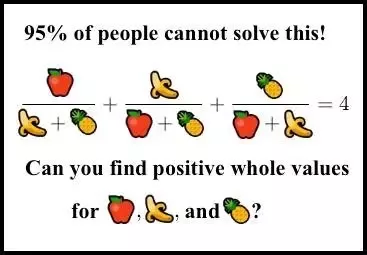
\includegraphics[width=0.5\textwidth]{img/positive_whole_values.png}
\end{center}

Now the original meme does not have the additional requirement of positive whole values, which do not really mean anything. If values refer to those of the complex field, then the problem is trivial, by the fundamental theorem of algebra. Alternatively, substituting $ b = 1 $ and $ c = 0 $ also gives a real quadratic solution $ a = 2 + \sqrt{3} $. The requirement of integers makes the problem slightly less trivial, but an observant eye would detect a trivial solution pretty easily, say $ a = 11 $, $ b = 4 $, and $ c = -1 $. This also generates a family of twelve related solutions, namely by flipping all the signs and permuting the roles of $ a, b, c $.

\subsection{Problem restatement}

The problem can be written as
\begin{equation}
\label{cubic}
\dfrac{a}{b + c} + \dfrac{b}{a + c} + \dfrac{c}{a + b} = 4, \qquad a, b, c \in \Z,
\end{equation}
where integers are considered for the sake of an easier argument, and checking $ a, b, c > 0 $ for a valid solution to $ \rb{\ref{cubic}} $ will be done later. This would have a family of \emph{trivial solutions}
$$
\begin{array}{lll}
\rb{a, b, c} & = & \rb{11, 4, -1} \\
& = & \rb{-11, -4, 1} \\
& = & \rb{1, -4, -11} \\
& = & \dots
\end{array}.
$$
Clearing denominators, $ \rb{\ref{cubic}} $ can be reduced to
\begin{equation}
\label{projective}
a^3 + b^3 + c^3 - 5abc - 3\rb{a^2b + ab^2 + a^2c + ac^2 + b^2c + bc^2} = 0, \qquad a, b, c \in \Z.
\end{equation}
There is an issue here needing to be addressed, that is the multiplication of denominators, which would be illegal if they are zero. This would now have several \emph{invalid solutions}
$$
\begin{array}{lll}
\rb{a, b, c} & = & \rb{1, -1, 0} \\
& = & \rb{-1, 1, 0} \\
& = & \rb{-1, 1, -1} \\
& = & \dots
\end{array}.
$$
These extraneous solutions, in a sense complete the space of solutions of $ \rb{\ref{cubic}} $, and will make the procedure described later much easier. Again, there is now a need to check that $ a + b, a + c, b + c > 0 $ for a valid solution to $ \rb{\ref{cubic}} $ later. This clearing of denominators is known as a \emph{birational transformation}.

\subsection{Dimensionality of solution space}

An immediate observation points out that $ \rb{\ref{cubic}} $ and $ \rb{\ref{projective}} $ are \emph{homogeneous}, which is to say that the polynomial defining it has terms of the same degree. For any given solution
$$ \rb{a, b, c} = \rb{a_0, b_0, c_0}, $$
scaling it by a non-zero rational number $ \lambda $ also produces another solution
$$ \rb{a, b, c} = \rb{\lambda a_0, \lambda b_0, \lambda c_0}, $$
which can be verified explicitly by collecting terms. These new solutions clearly do not help in understanding the space of solutions to $ \rb{\ref{projective}} $, as they do not contribute in the generation of more solutions. It would thus be conducive to consider the equivalence class of solutions
$$ \rb{a, b, c} = \sb{a_0, b_0, c_0}, $$
defined by the equivalence relation
$$ \rb{a_0, b_0, c_0} \sim \rb{a_0', b_0', c_0'} \qquad \iff \qquad \rb{a_0, b_0, c_0} = \rb{\lambda a_0', \lambda b_0', \lambda c_0'} \ \text{for some} \ \lambda \in \Q^*. $$
Considering only the equivalence classes where $ c \ne 0 $, a natural representative can be designated to each of them. For instance, letting $ \lambda = \tfrac{1}{c} $ for any $ c $ will force $ c = 1 $ in each equivalence class, cutting down $ \rb{\ref{projective}} $ to one of only two variable dimensions $ a $ and $ b $, both of which can be arbitrary rational numbers. In other words, $ \rb{\ref{projective}} $ only pretends to have three-dimensional when it actually behaves more like two-dimensional, plus the case where $ c = 0 $. To respect this property, $ \rb{\ref{projective}} $ can and will be rewritten in the form
\begin{equation}
\label{affine}
a^3 + b^3 + 1 - 5ab - 3\rb{a^2b + ab^2 + a^2 + a + b^2 + b} = 0, \qquad a, b \in \Q,
\end{equation}
which is cubic of two variables. This is known as the \emph{dehomogenisation} of a homogeneous equation.

\section{Elliptic curves}

\subsection{Informal definition}

\emph{Elliptic curves} are a family of homogeneous cubic equations with the aforementioned property, where they have three variables, yet in a sense behave more like two-dimensional. These are usually represented by an equation of the form
$$ y^2 = x^3 + Ax + B, $$
where $ A $ and $ B $ are in some field. There is an additional requirement that $ 4A^3 + 27B^2 \ne 0 $, which is to ensure that the graph of the equation is drawn without any kinks. Elliptic curves are typically one of the simplest non-trivial structures in algebraic geometry, and are used widely in and out of applications.
\begin{itemize}
\item For instance, one of the \emph{Millennium Prize Problems} set by the \emph{Clay Mathematics Institute} is the \emph{Birch and Swinnerton-Dyer conjecture}, which questions properties of the \emph{rank} of a rational elliptic curve.
\item In Wiles' proof of \emph{Fermat's last theorem}, he deduced a contradiction to \emph{Fermat's equation} having any non-trivial solutions, by asserting the existence of an impossible \emph{modular elliptic curve}.
\item There are also extremely efficient algorithms of performing primality testing and integer factorisation involving elliptic curves, both of which considered state-of-the-art techniques.
\item Finally, the advent of \emph{elliptic curve cryptography} also allowed for relatively small keys for encryption and decryption schemes, revolutionalising many cryptosystems.
\end{itemize}

\subsection{Formal definition}

An \emph{elliptic curve} over a \emph{perfect field} $ K $ is a \emph{smooth projective plane algebraic curve} $ E $ of \emph{genus one} with a \emph{flex $ K $-rational base point} $ \OO_E $.
\begin{itemize}
\item An \emph{algebraic curve} is an \emph{algebraic variety of dimension one}, which is to say that it is the space of solutions to one specified equation.
\item Being embedded in the \emph{projective plane} refers to the notion of having three variables but behaving more like two-dimensional, through considering equivalence classes of solutions.
\item \emph{Smoothness} is a degeneracy condition that avoids any nodes, cusps, self-intersections, or isolated points.
\item \emph{Genus one} basically means a degree three cubic curve via the \emph{genus-degree formula}, but the term is used here as the usual invariant for algebraic curves. It can be defined algebraically via a fundamental theorem in algebraic geometry known as the \emph{Riemann-Roch theorem}, but it was motivated from topology, where the \emph{topological genus} refers to the number of holes in some surface. In this case, a complex elliptic curve can be thought of as a \emph{Riemann surface}, which can be deformed into a torus with one hole via its \emph{fundamental parallelogram}.
\item An additional requirement of a base point distinguishes elliptic curves from general cubic curves. Elliptic curves are often considered over the \emph{algebraic closure} of its base field, but \emph{$ K $-rationality} ensures that the base point has coordinates in $ K $. Being a \emph{flex} means that the \emph{intersection multiplicity} of its tangent with the ambient curve is exactly three, which can be informally thought of as slight perturbations of its tangent locally giving exactly three intersections with the ambient curve. This last condition is not usually considered by virtue of the \emph{chord-tangent method}, but it simplifies definitions.
\item Finally, \emph{perfectness} of the base field is also a degeneracy condition that requires every \emph{algebraic extension} to be \emph{separable}.
\end{itemize}
Fortunately, these definitions can be translated, again via the \emph{Riemann-Roch theorem}, to say that any elliptic curve over $ \Q $ is of the form
$$ \cb{\rb{x, y} \in \Q^2 \mid x^3 + Ax + B} \cup \cb{\OO}, $$
for some $ A, B \in \Q $ such that its \emph{discriminant} $ 4A^3 + 27B^2 $ is non-zero, where $ \OO = \sb{0, 1, 0} $ is a formal symbol representing an invalid solution. This definition also works for any perfect field $ K $ of characteristic $ char\rb{K} \notin \cb{2, 3} $.

\subsection{Weierstrass equations}

With this in mind, $ \rb{\ref{affine}} $ can also be transformed in several steps into a standard form of an elliptic curve, via algorithms detailed in \ref{weierstrass} and \ref{laska}. Coincidentally, it happens that the curve given by $ \rb{\ref{affine}} $ is smooth, so that the following transformations are actually \emph{isomorphisms of algebraic varieties}. This does not matter in the grand scheme of things, as otherwise they are birational transformations that would still preserve most of the relevant structure in consideration.
\begin{itemize}
\item The initial transformation sends any invalid solution, say $ \sb{1, -1, 0} $, to the \emph{point at infinity} $ \OO $, and its tangent, $ c = 6a + 6b $, to the \emph{line at infinity} $ z = 0 $. This could be done by choosing a different point in the tangent, say $ \sb{1, 0, 6} $, and sending it to different point in the line at infinity, say $ \sb{1, 0, 0} $. A third linearly independent finite point, say $ \sb{1, 0, 0} $, can then be sent to a third linearly independent finite point, say $ \sb{0, 0, 1} $, to allow the \emph{projective transformation} matrix to be invertible. In other words, the change of variables is induced by a matrix in $ PGL_3\rb{\Q} $. This produces the cubic curve
$$ \cb{\rb{x, y} \in \Q^2 \mid 6y^2 + 6xy + 6y = -91x^3 + 141x^2 + 15x - 1} \cup \cb{\OO}. $$
This is followed by an appropriate transformation $ z \mapsto -\tfrac{6}{91}z $ to give a \emph{long Weierstrass equation}
$$ \cb{\rb{x, y} \in \Q^2 \mid y^2 + xy - \tfrac{91}{6}y = x^3 + \tfrac{47}{2}x^2 - \tfrac{455}{12}x - \tfrac{8281}{216}} \cup \cb{\OO}. $$
This elliptic curve is in fact a \emph{minimal model} with smallest possible discriminant.
\item The next transformation traces a simplified version of \emph{Laska's algorithm} for rational elliptic curves, which imposes several conditions on the coefficients of the equation after applying isomorphisms. This produces a unique \emph{restricted} and \emph{integral} minimal model
$$ \cb{\rb{x, y} \in \Q^2 \mid y^2 + xy + y = x^3 - 234x + 1352} \cup \cb{\OO}, $$
which also has small integral coefficients. This particular form can also be looked up in the \emph{$ L $-functions and modular forms database} under the label $ 910.a4 $.
\item Another transformation, which works for fields of characteristic not two, completes the square with the transformation $ y \mapsto -\tfrac{1}{2}x + y - \tfrac{1}{2}z $ to give a \emph{medium Weierstrass equation}
$$ \cb{\rb{x, y} \in \Q^2 \mid y^2 = x^3 + \tfrac{1}{4}x^2 - \tfrac{467}{2}x + \tfrac{5409}{4}} \cup \cb{\OO}, $$
which is a minimal model but does not have integral coefficients. Clearing denominators,
$$ \cb{\rb{x, y} \in \Q^2 \mid y^2 = x^3 + 109x^2 + 224x} \cup \cb{\OO} $$
is an integral model but will not have minimal discriminant anymore.
\item Finally, another transformation, which works for fields of characteristic not two or three, completes the cube with the transformation $ x \mapsto x - \tfrac{1}{12}z $ to give a \emph{short Weierstrass equation}
$$ \cb{\rb{x, y} \in \Q^2 \mid y^2 = x^3 - \tfrac{11209}{48}x + \tfrac{1185157}{864}} \cup \cb{\OO}, $$
which is a minimal model but does not have integral coefficients. Clearing denominators again,
$$ \cb{\rb{x, y} \in \Q^2 \mid y^2 = x^3 - 302643x + 63998478} \cup \cb{\OO}, $$
is an integral model but will not have minimal discriminant anymore.
\end{itemize}
All of these transformations preserve the \emph{$ j $-invariant} of the rational elliptic curve, a quantity that characterises the isomorphism classes of elliptic curves over algebraically closed fields. The focus now shifts to the simplest model of the same elliptic curve, namely the equation representing the last curve,
\begin{equation}
\label{elliptic}
y^2 = x^3 + Ax + B, \qquad A = -302643, \qquad B = 63998478.
\end{equation}
The overall transformation can be recorded in one change of variables
$$
\begin{cases}
a = \tfrac{1}{72}x + \tfrac{1}{216}y - \tfrac{277}{24} \\
b = \tfrac{1}{72}x - \tfrac{1}{216}y - \tfrac{277}{24} \\
c = \tfrac{1}{6}x - \tfrac{95}{2}
\end{cases}
\qquad
\begin{cases}
x = \dfrac{1710a + 1710b - 831c}{6a + 6b - c} \\
y = \dfrac{-9828a + 9828b}{6a + 6b - c}
\end{cases},
$$
which are clearly inverses.

\subsection{Group law}

An elliptic curve is also an \emph{abelian variety of dimension one}, which makes it an \emph{algebraic group}. In other words, an abelian group could be defined over points on the elliptic curve. The following definition for $ \rb{\ref{elliptic}} $ will suffice for most purposes, but more complicated definitions exist for fields of characteristic two and three.
\begin{itemize}
\item The identity point is $ \OO \in E $.
\item The inverse of a point is obtained by reflecting the point about the $ x $-axis, where $ -\rb{x, y} = \rb{x, -y} $.
\item The sum of two points is obtained by inverting the third point of intersection between the curve and the line joining the two points, where
$$ P + Q =
\begin{cases}
S & P = \rb{x, y}, \ Q = \rb{x', y'}, \ x \ne x' \\
R & P = Q = \rb{x, y}, \ y \ne 0 \\
P & Q = \OO \\
\OO & P = Q = \rb{x, 0}
\end{cases},
$$
$$ S = \rb{\tfrac{\rb{A + xx'}\rb{x + x'} + 2\rb{B - yy'}}{\rb{x - x'}^2}, \tfrac{\rb{Ay' - x'^2y}\rb{3x + x'} + \rb{x^2y' - Ay}\rb{x + 3x'} - 4B\rb{y - y'}}{\rb{x - x'}^3}}, $$
$$ R = \rb{\tfrac{x^4 - 2Ax^2 - 8Bx + A^2}{4y^2}, \tfrac{x^6 + 5Ax^4 + 20Bx^3 - 5A^2x^2 - 4ABx - A^3 - 8B^2}{8y^3}}. $$
\end{itemize}
The explicit equations here describe the four cases involved and show that it is possible to program the computations despite its geometric definition. For it to be well-defined, there are several things to check.
\begin{itemize}
\item Firstly, point addition needs to be well-defined over the base field. \emph{B\'ezout's theorem} states that two projective algebraic curves $ C $ and $ D $ over an algebraically closed field intersect at $ \deg C\deg D $ points counted with intersection multiplicity. It follows that the third point of intersection in the above definition is well-defined over the algebraic closure of the base field. Since the explicit equations are all rational functions, this point would also be well-defined over the base field.
\item Next, commutativity of point addition holds by symmetry of its definition.
\item Finally, associativity of point addition involves more complications and is practically the only non-trivial axiom to check. There are at least three ways to verify this fact.
\begin{itemize}
\item An extremely tedious approach considers all possible cases in the explicit equations to be verified sequentially. This could be done with a computer algebra system that might take several hours.
\item A more geometric approach considers ten points in \emph{general position} without loss of generality. The \emph{Cayley-Bacharach} theorem states that three projective algebraic cubic curves over an algebraically closed field that coincide at eight points counted with intersection multiplicity would coincide at the ninth point given by B\'ezout's theorem. Now consider the following diagram, where $ P, Q, R, S \in E $ are points in general position.
$$
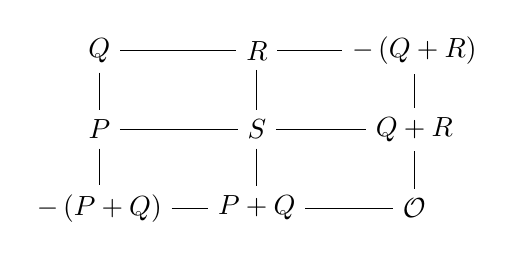
\begin{tikzpicture}
\node(Q) at (-2, 1) {$ Q $};
\node(R) at (0, 1) {$ R $};
\node(QR') at (2, 1) {$ -\rb{Q + R} $};
\node(P) at (-2, 0) {$ P $};
\node(S) at (0, 0) {$ S $};
\node(QR) at (2, 0) {$ Q + R $};
\node(PQ') at (-2, -1) {$ -\rb{P + Q} $};
\node(PQ) at (0, -1) {$ P + Q $};
\node(O) at (2, -1) {$ \OO $};
\draw (Q) -- (R) -- (QR');
\draw (P) -- (S) -- (QR);
\draw (PQ') -- (PQ) -- (O);
\draw (Q) -- (P) -- (PQ');
\draw (R) -- (S) -- (PQ);
\draw (QR') -- (QR) -- (O);
\end{tikzpicture}
$$
The union of the three horizontal lines and the union of the three vertical lines give two cubic curves, both of which passes through eight points in the ambient elliptic curve. It follows that $ -\rb{P + \rb{Q + R}} = S = -\rb{\rb{P + Q} + R} $, proving associativity.
\item A more algebraic approach considers the \emph{Picard group} $ Pic^0\rb{E} $ of an elliptic curve $ E $, which is in set-theoretic bijection with $ E $ via the \emph{summation map}. This also induces an isomorphism of abelian groups that coincides with the geometric definition, which has associativity as a consequence.
\end{itemize}
\end{itemize}
This completes the proof of the group law of an elliptic curve.

\section{Procedure}

\subsection{Generation algorithm}

The following algorithm then details the procedure to generate new solutions from old solutions.
\begin{itemize}
\item Choose an initial solution for
$$ a^3 + b^3 + c^3 - 5abc - 3\rb{a^2b + ab^2 + a^2c + ac^2 + b^2c + bc^2} = 0, \qquad a, b, c \in \Z. $$
\item Apply the change of variables
$$
\begin{cases}
x = \dfrac{1710a + 1710b - 831c}{6a + 6b - c} \\
y = \dfrac{-9828a + 9828b}{6a + 6b - c}
\end{cases}.
$$
\item Compute multiples of point in
$$ y^2 = x^3 + Ax + B, \qquad \rb{x, y} \in \Q^2. $$
\item Apply the change of variables
$$
\begin{cases}
a = \tfrac{1}{72}x + \tfrac{1}{216}y - \tfrac{277}{24} \\
b = \tfrac{1}{72}x - \tfrac{1}{216}y - \tfrac{277}{24} \\
c = \tfrac{1}{6}x - \tfrac{95}{2}
\end{cases}.
$$
\item Terminate or repeat.
\end{itemize}

\subsection{Computation failure}

It is entirely possible that the algorithm fails for a few reasons. The solutions obtained may not have positive whole values, and running the procedure over and over again may never result in any such solutions. Such a failure occurs when considering the multiples of any invalid solution, such as
$$ \rb{a, b, c} = \rb{-1, 1, -1}. $$
Applying the change of variables gives
$$ \rb{x, y} = \rb{831, 19656}, $$
so consider the cyclic subgroup generated by this point.
\begin{align*}
1\rb{x, y} & = \rb{831, 19656}, \\
2\rb{x, y} & = \rb{363, 1404}, \\
3\rb{x, y} & = \rb{327, 0}, \\
4\rb{x, y} & = \rb{363, -1404}, \\
5\rb{x, y} & = \rb{831, -19656}, \\
6\rb{x, y} & = \OO.
\end{align*}
The algorithm hits a \emph{torsion subgroup} of order six, which will never result in any valid solutions, no matter the number of repetitions.

\subsection{Computation success}

Fortunately, this is not always the case, provided no invalid solutions are chosen in the beginning. Considering any trivial solution will eventually result in success, such as for
$$ \rb{a, b, c} = \rb{11, 4, -1}. $$
Applying the change of variables gives
$$ \rb{x, y} = \rb{291, -756}, $$
so again consider the cyclic subgroup generated by this point. Duplicating the point once gives
$$ 2\rb{x, y} = \rb{\tfrac{22107}{49}, -\tfrac{1506492}{343}}, $$
where reverting the change of variables would give
$$ \rb{a, b, c} = \rb{-8784, 5165, 9499}. $$
This is in fact a point of infinite order by the \emph{Nagell-Lutz theorem}, so continuing would be conducive. Triplicating the point once gives
$$ 3\rb{x, y} = \rb{-\tfrac{2694138}{11881}, -\tfrac{14243306490}{1295029}}, $$
where reverting the change of variables would give
$$ \rb{a, b, c} = \rb{679733219, -375326521, 883659076}. $$
Triplicating this point once more gives
\begin{align*}
9\rb{x, y} = (& \tfrac{3823387580080160076063605209061052603963389916327719142}{13514400292716288512070907945002943352692578000406921} \\
& -\tfrac{1587622549247318249299172296638373895912313166958011719500537215259315694916502670}{1571068668597978434556364707291896268838086945430031322196754390420280407346469}),
\end{align*}
where reverting the change of variables would finally give the required solutions. This last point is said to have a large \emph{height}, which measures the complexity of the coordinates from the numerators and denominators.

\subsection{Miscellaneous considerations}

The general equation being considered in the original paper was
$$ \dfrac{a}{b + c} + \dfrac{b}{a + c} + \dfrac{c}{a + b} = N, \qquad a, b, c \in \N^*, \qquad N \in \Z, $$
which considers a similar procedure as aforementioned. The torsion subgroup and rank of the elliptic curves \emph{birationally equivalent} to these cubic curves can be computed systematically, such that, in conjunction with \emph{Mordell's theorem}, they are all isomorphic as abelian groups to the finitely generated abelian group
$$ \Z^r \oplus
\begin{cases}
\Z / 2\Z \oplus \Z / 6\Z & N = 2 \\
\Z / 6\Z & \text{otherwise}
\end{cases},
\qquad
r \in \N^*.
$$
The curve for $ N = 4 $ has $ r = 1 $, which ensures the existence of a point of infinite order, hence giving a termination point for the algorithm. The termination point detailed above does indeed give the smallest solution, which can be proven with the theory of heights. It is entirely possible that $ r = 0 $, or that $ r > 0 $ but yet no positive whole solutions exist no matter the number of repetitions. Such is the case for all odd $ N $, which can be proven using ad-hoc congruences. For even $ N $, it is also possible that no solutions exist, such is the case for $ N = 8 $. When there are solutions, they may take arbitrarily large point multiples to obtain, and the resulting solution may have arbitrarily large positive values. In the case for $ N = 178 $, the corresponding initial point has to be multiplied over a hundred thousand times, and the resulting solution has over four hundred million digits.

\section{References}

\begin{enumerate}[label={[\arabic*]}]
\item A Amit's Quora answer on \emph{How do you find the positive integer solutions to} \label{quora}
$$ \dfrac{x}{y + z} + \dfrac{y}{z + x} + \dfrac{z}{x + y} = 4? $$
\item A Bremner and A Macleod's 2014 paper on \emph{An unusual cubic representation problem} \label{aucrp}
\item J Silverman's 1986 book \emph{The arithmetic of elliptic curves} \label{aec}
\item R Hartshorne's 1977 book on \emph{Algebraic geometry} \label{ag}
\item N Duif's 2011 implementation on \emph{Transforming a general cubic elliptic curve equation to Weierstrass form} \label{weierstrass}
\item M Laska's 1982 paper on \emph{An algorithm for finding a minimal weierstrass equation for an elliptic curve} \label{laska}
\end{enumerate}

\end{document}